\section{Implementation}\label{implementation}

This section describes the implementation process. The design highlighted the usage of the dashboard through its personas and scenarios, while the low fidelity mockups gave an early glance at its appearance. At its core, the strength of the application revolves around its extensibility and usability. Therefore, a lot of thought went into choosing the best libraries to provide these features.

First, an overview of the entire application is given, after which we go into more detail. The dashboard consists of two major parts common to web development. The back end is described first. This section covers explains the reasoning behind the chosen technology stack and the general structure. We also specify the back end structures and REST API calls for each module and component which the front end has access to. For the front end, we explain how the Polymer 3 library supports our modular design and its underlying principles. Hereafter, other libraries used during the implementation, the general front end structure, and the resulting dashboard and its modules are explained. 

It is without question that during the implementation small changes were made to the design. These changes are documented for both parts. During the entire development process, only basic authentication was implemented. The implementation of standards, privacy rules, and security techniques do not contribute towards the goal of the dashboard we defined in the design section. Therefore, no effort was put in these topics.

    \subsection{Overview}

    The first major choice that was made, was the type of application to develop: a native application or a web application. It was a relative simple choice, but nonetheless an important one. Native applications are developed, in most cases, for one type of operating system. If a vendor wants to support both Android and iOS devices, two separate applications need to be developed. This requires more developers to not only create the application, but also to maintain it. Another drawback of native applications is the update process. This process often requires the reinstallation of the entire application, which is very disruptive and difficult to do in a care setting.

    Web applications saw a surge in popularity. Compared to their native counterparts, web applications today are becoming increasingly similar in terms of functionality and design. Office Online from Microsoft is a good example showcasing this, which features many functions found on the desktop versions of the Office Suite. While these web applications also require updates, these happen on the server side. When the user refreshes the web page, the latest version of the application is automatically retrieved. This simplifies the roll-out process significantly. Also, all operating systems that support web browsers, are capable of running this type of applications. This includes mobile devices. As a result, developers only have to develop one application. However, the variation in screen resolutions and aspect ratios calls for a responsive design.

    With this in mind, the choice to create a web application was evident. Users can view the dashboard regardless of the device they use, without sacrificing functionality. It should be noted that complex operations will not fit easily into a web application. The strength of web apps also leads to its major drawback: poor performance. A native application can draw much more computational power from the device it was made for. To transfer the computation burden to the server is also not a viable solution as this puts additional strain on the network. In case of real-time applications, latency becomes an issue due to continuous data transfer. However, the dashboard application should not experience any performance issues as the modules that were defined in section~\ref{app_specification} do not require complex operations.

    \begin{figure}[!t]
        \centering
        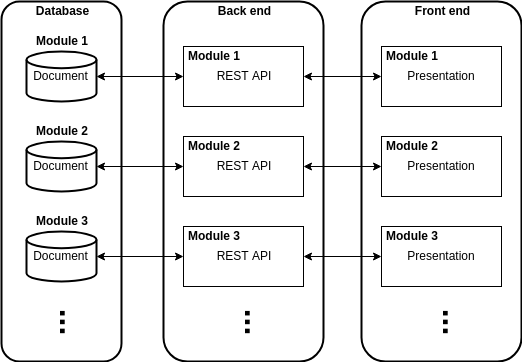
\includegraphics[width=1\textwidth]{chapters/4_implementation/structure}
        \caption{The communication flow by which every module communicates.}\label{fig:structure}
    \end{figure}

    A typical web application consists of two parts: the back end and the front end. In software engineering principles, these refer to the separation of the data access layer and the presentation layer of the web application. For example, the back end fetches data requested by the front end. In turn, the front end presents the retrieved data towards the user. Due to the modular design of the dashboard, each module needs to have its own back and front end structures, visualized by figure~\ref{fig:structure}. As the figure indicates, there is no direct interaction between the modules, which facilitates low coupling. The next sections describe the back end and front end in detail. Changes made to the design from section~\ref{design} are explained.

    \subsection{Back end}

    \begin{figure}[!t]
        \centering
        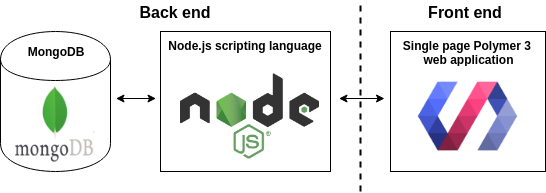
\includegraphics[width=1\textwidth]{chapters/4_implementation/tech}
        \caption{The three core technologies used to build the application.}\label{fig:tech}
    \end{figure}

    The back end is responsible for everything related to the management of the data present in the dashboard application. It is here that the logic is defined to add, update, or remove records from the database based on the requests it received from the front end. The back end exposes a REST API which determines which requests the front end can send.

    This section gives a detailed description of how the back end part of the dashboard was implemented. First, we go over the chosen technology stack after which we explain the back end structure. To close, each component present in the back end is briefly described.

        \subsubsection{Technology stack}

        Figure~\ref{fig:tech} shows the three core technologies used to develop the application. The back end was built using Node.js and MongoDB\@. We now give a brief explanation of what each back end component tries to achieve and why it was chosen.

            \subsubsubsection{Node.js}

            The back end server forms the heart of the dashboard application and Node.js was the preferred choice to implement it. Node.js (or simply Node) is a Java-Script runtime built on Google Chrome's V8 JavaScript engine~\cite{NodeJS}. Node.js avoids the classic thread-based approach of concurrency, which is relatively inefficient and can be very difficult to use. Instead, it provides concurrency via a single event loop that can support thousands of simultaneous connections, using non-blocking I/O calls. Node also has the added bonus of streamlining web development to the use of a single language.
            
            The main reason Node.js was chosen, was due to the very large collection of packages that is available through the Node Package Manager (npm). For example, the Express package is only available via Node. This package was of significant help during the entire development process. Also, documentation is easily found thanks to the very large community that develops with Node.

            \subsubsubsection{MongoDB} 
            
            A SQL database is table-based, whereas MongoDB is document-based. This type of structure enables highly flexible data schemas, as new data fields can be added without affecting existing rows. This is especially useful when a new data structure from a 3rd vendor needs to be added to the database. This supports the dashboard's goal of simple extensibility. Also, the developers of MongoDB officially support Node.js.

            \subsubsubsection{Node packages}

            Node allows developers to easily install a broad selection of packages. We now discuss the packages that were used for the development of the back end. These served many purposes, such as routing, encryption, logging, and request body parsing. 

                \paragraph{Mongoose} Using Node without a library to communicate with the MongoDB is very difficult, as data validation and casting must be written manually. By installing the Mongoose, a MongoDB object modeling package, this will be taken care of. Via the package we can define data schemas and its parameters. Hereafter, a data model is created by compiling the schema. It is now possible to create MongoDB documents in a very similar fashion to object-oriented programming, which encapsulates the more complex inner workings of MongoDB\@. The entire database is constructed via these models.

                \paragraph{Express} Express is a Node.js web application framework, which helps with the management of routing, connecting middleware, handling requests and others. It helps to organize a web application on the server side into a MVC architecture. Also, Express makes the creation of a REST API server a much faster process compared to vanilla Node. Since we need to transfer data from MongoDB to our front end via a REST API, this framework is absolutely essential.

                \paragraph{Bcrypt \& JSON Web Tokens} Basic encryption is provided by the bcrypt package. Whenever a user registers, the password is hashed and then stored into MongoDB via Mongoose. In case the user successfully authenticates, the JSON Web Tokens package generates a token based on the login name, user id, clearance level, and a secret phrase. This token is sent back to the front end and must be embed into every future request. After one hour, the token expires and the user must authenticate again.

                \paragraph{Other} The body-parser package helps as its name implies with parsing request bodies. This package is connected to Express as middleware, since it captures the request and parses it before it lands in the developer's hands. Morgan is another helpful package which logs all requests made to the server. As such, it is a helpful debugging tool. Last, but certainly not least, is the nodemon package. Nodemon detects changes in a Node.js project. If changes are found, nodemon restarts the application automatically to apply these changes.


        \subsubsection{Structure}
        
        As mentioned before, the Express framework can help with organizing a web application into a MVC architecture. The entire dashboard prototype is built around this architecture. The MVC architecture consists of three parts:
        \begin{itemize}
            \item Model: the part that manages the data and receives input from the controller. This is handled by Mongoose.
            \item View: the view presents the model or in other words, the data. The front end is our view, which is a Polymer 3 server.
            \item Controller: the controller handles incoming requests from the view. Hereafter it calls upon the model to get the desired data, which it then returns to the view. This is done on the back end Node.js server with the help of Express.
        \end{itemize}

        \noindent Every module present in the back end has three files of the same name, but each saved into the following folders: controller, models, and routes. They are connected as follows:
        \begin{myenumerate}
            \item The front end sends a request to a certain route. Express checks this route and sees that the file \texttt{routes/patient.js} uses it. 
            \item \texttt{routes/patient.js} has every possible API endpoint mapped to a controller function which executes certain logic to retrieve data. All these controller functions are found in the \texttt{controller/patient.js} file.
            \item Last, certain logic gets executed depending on which controller function is called. The controller calls the Mongoose model to perform certain actions on the database, which is defined in \texttt{models/patient.js}.
            \item Depending on the operation, the controller can send data retrieved from the model back to the view. This transaction does not pass by the router.
        \end{myenumerate}

        \noindent In order to extend the dashboard application, these three files need to be created for each component. More concrete steps are given in appendix TODO.

        \paragraph{Routing} The routes defined in the back end follow a simple structure. All modules that do \emph{not} retrieve patient data, start at the root endpoint: \texttt{/}. For example, to log in, the front end needs to send a POST request with the credentials stored in its body to the following endpoint: \texttt{/login}. In case a module does retrieve patient data, the endpoint is always prefixed with the patient id. Suppose the front end wants to retrieve all allergies of a patient, then it sends a GET request to  the following endpoint: \texttt{/uniquepatientid/allergy/}. The file \texttt{routes/patient.js} will have an entry to forward all sub-routes that start with ``allergy'' to the routes defined in \texttt{routes/modules/allergy.js}.

        \subsubsection{Components and dashboard modules}

        % files of same name found in controller, models, and routes

            \paragraph{Clinician}

            \paragraph{Layout}

            \paragraph{Import}

            \paragraph{Patient}

            \subsubsubsection{Dashboard modules}

                \paragraph{Prescription}

                \paragraph{Allergy}

                \paragraph{Vaccination}

                \paragraph{Workflow}

                \paragraph{Checklist}

                \paragraph{History}

                \paragraph{Telemonitoring}

    \subsection{Front end}

    The front end serves as the face of the dashboard application and is more complex than its back end counterpart. Throughout the lengthy implementation phase several were made, which required some work to be redone, but in the end promotes better extensibility and usability. 
    
    A modular dashboard was built using the Polymer 3 framework in combination with several libraries. The topics web components and shadow DOM are very important in realizing loosely coupled and highly cohesive modules, which is why it is important to understand them. After the used libraries are explained, the structure of the front end is described. To close, the end result is shown via various screenshots of the dashboard and its modules.

        \subsubsection{Polymer 3}

        Polymer is an open-source library that provides a set of feature for creating web components. These web components work similar to standards DOM elements such as \texttt{<h1>Title</h1>}. The library is developed by Google and contributors. Several Google services such as YouTube and Google Earth were developed with Polymer. We now explain two principles that lay at the heart of the library.

            \subsubsubsection{Web Components}

            HTML provides us with standard elements such as \texttt{h1} and \texttt{img}. Web Components allows the developer to create custom elements which are used in the same manner as the ones HTML provides. Suppose a calendar Web Component was created, a developer could add the element to any web page as follows: \texttt{<calendar></calendar>}. The actual definition of the calendar module resides in another file which is imported on the page where it will be used. This approach promotes the creation of reusable components, and above all, easy integration which is a primary goal of our dashboard application. At the heart of Web Components is the shadow DOM\@.

            \subsubsubsection{Shadow DOM}

            We assume the reader is familiar with the DOM concept. The shadow DOM can be seen as a scoped subtree inside a custom element. The root of this subtree is called the shadow root. The structure, styling, and behavior of the children within the shadow DOM do not affect any elements outside of it. Therefore, the appearance and functionality of the custom element is encapsulated and hidden at the document level. Only events fired by elements in the shadow DOM can be pickup outside the shadow DOM boundary. This idea of encapsulation is important for our approach towards the dashboard, as each module is responsible for its own appearance and functionality. Developers of custom modules should not need to worry about what happens outside of the shadow DOM\@.

        \subsubsection{Libraries}

        The dashboard must support resizing, and dragging \& dropping of modules. To realize this, several libraries were compared to each other. After careful consideration, choices were made. During this section the libraries used to create the front end functionality are described.

            \paragraph{Packery \& Draggabilly} Packery was chosen to create the grid in which the modules are placed. It features algorithms to minimize whitespace and gapless layouts. As items are added and removed from the grid, Packery reorders the grid. To make the items draggable, an additional library supported by Packery must be used, called Draggabilly. 

            \paragraph{Interact.js} This library implements JavaScript drag and drop, resizing and multi-touch gestures for modern browsers. However, Draggabilly already provides drag and drop functionality. Since Interact.js is not supported by Packery, Draggabilly can not be removed. Therefore, Interact.js serves as the library that implements the resizing functionality for the modules.

            \paragraph{Other} moment c3

        \subsubsection{Structure}

        \subsubsection{Dashboard}

        \subsubsection{Modules}

            \subsubsubsection{Prescription}

            \subsubsubsection{Allergy}

            \subsubsubsection{Vaccination}

            \subsubsubsection{Workflow}

            \subsubsubsection{Checklist}

            \subsubsubsection{History}

            \subsubsubsection{Telemonitoring}
